\documentclass[12pt]{article}

\usepackage{sbc-template}
\providecommand{\gls}[1]{\textnormal{\textsc{#1}}}
\providecommand{\Gls}[1]{\textnormal{\textsc{#1}}}

\usepackage{amsmath}
\usepackage[utf8]{inputenc}
\usepackage[brazil]{babel}
\usepackage{graphicx,url}
\usepackage{tabularx}
\usepackage{booktabs}
\usepackage{array}
\usepackage{placeins}

\newcolumntype{Y}{>{\raggedright\arraybackslash}X}

\sloppy
\raggedbottom

% Remove address row: SBC's \@maketitle inserts \inst{\instnum}=$^1$ before \@address
\makeatletter
\def\@maketitle{\newpage
 \begin{center}
   \vspace*{-.7cm}
   {\XVIPT\bf\@title\par}
   \vglue 6pt plus 3pt minus 3pt
   {\normalsize
    \textbf{\begin{tabular}[t]{c}\@author\end{tabular}}\par}
   \vglue 6pt plus 3pt minus 3pt
 \end{center}\par
}
\makeatother

\title{Pipeline Interpretável para Detecção de Doenças Foliares em Tomateiro com Inferência em Borda via Rust/ONNX}

\author{}

\address{}

\begin{document}

\maketitle

\begin{abstract}
This work presents a low-cost smart indoor garden for tomato cultivation
integrating embedded sensing, actuation, and AI for foliar disease detection.
An \gls{ESP32}-S3 with \gls{OV2640} monitors temperature, humidity, and soil
moisture, automating irrigation and ventilation; leaf images are forwarded to
a Rust/Axum inference server with ONNX Runtime. The classical pipeline applies
\gls{HSV}-based segmentation---removing the white PlantVillage background
($S\approx0$)---and extracts a 188-dimensional feature vector (Haralick,
Zernike, \gls{LBP}, Hu moments, colour histograms, shape descriptors). Among
\gls{XGBoost}, SVM, and Random Forest under StratifiedGroupKFold, XGBoost
achieved macro F1 96.19\% (MCC 0.9607) on a 10-class test set of 4{,}803
samples; MobileNetV3-Small reached 99.02\% as a deep baseline. In a controlled
benchmark ($N=100$), Rust achieved median latency 13.2\,ms vs.\ 24.5\,ms for
Python/Flask ($p<0.001$, Mann-Whitney~U), with 82\% lower memory footprint,
enabling edge deployment on resource-constrained hardware.
\end{abstract}

\begin{resumo}
Este trabalho apresenta uma horta indoor inteligente de baixo custo para o
cultivo de tomateiro, integrando sensoriamento embarcado, atuação e IA para
detecção de doenças foliares. Um \gls{ESP32}-S3 com câmera \gls{OV2640}
monitora temperatura, umidade e solo, automatizando irrigação e ventilação;
imagens foliares são encaminhadas a um servidor Rust/Axum com ONNX Runtime.
O pipeline clássico aplica segmentação \gls{HSV}---removendo o fundo branco
do PlantVillage ($S\approx0$)---e extrai um vetor de 188 atributos (Haralick,
Zernike, \gls{LBP}, Hu, histogramas de cor, descritores de forma). Entre
\gls{XGBoost}, SVM e Random Forest com StratifiedGroupKFold, o XGBoost obteve
macro F1 96,19\% (MCC 0,9607) em conjunto de teste de 4.803 amostras e 10
classes; a MobileNetV3-Small atingiu 99,02\% como baseline profunda. Em
benchmark controlado ($N=100$), o Rust apresentou latência mediana de
13,2\,ms contra 24,5\,ms do Python/Flask ($p<0{,}001$, Mann-Whitney~U), com
82\% menos memória, viabilizando implantação em hardware de borda.
\end{resumo}

\section{Introdução}

A agricultura contemporânea enfrenta o desafio de elevar a produtividade com
uso mais eficiente de água e energia. No cultivo do tomateiro, essa necessidade
é ampliada pela elevada exigência hídrica e pela suscetibilidade a doenças
foliares, exigindo monitoramento contínuo do ambiente e do estado
fitossanitário das plantas. Muitas soluções disponíveis ainda apresentam
infraestrutura complexa, o que limita sua adoção por pequenos produtores e
iniciativas de agricultura urbana. Nesse contexto, sistemas automatizados
tornam-se relevantes para ampliar a adoção da agricultura digital e de
precisão.

A literatura recente aponta essa convergência entre automação agrícola,
\gls{IoT} e visão computacional. Sensores de umidade do solo,
microcontroladores e algoritmos de manejo hídrico têm apresentado ganhos de
produtividade e economia de água e
energia~\cite[p.~106--109]{azevedo2025}; sistemas com sensores e atuadores
também têm mostrado resultados positivos no
tomateiro~\cite[p.~182--185]{ARAUJO2023}, e estudos adicionais reforçam a
influência do manejo hídrico no crescimento vegetativo e na
produtividade~\cite{campos2020,Silva2025}. No contexto de estufas inteligentes, sensores, atuadores e plataformas
\gls{IoT} têm sido empregados para controle ambiental~\cite{Borba2022,Leite2022,Costa2020,Ouhami2021},
enquanto técnicas de \gls{IA} e Visão Computacional alcançam elevados níveis
de acurácia na classificação de doenças foliares em tomateiro, com redes
neurais convolucionais e abordagens
híbridas~\cite{Paul2023,Kebir2024,Wang2024,Mac2024}.

Diante desse cenário, este trabalho propõe uma horta inteligente para o
cultivo de tomateiro integrando automação agrícola, \gls{IoT} e \gls{IA}. O
sistema utiliza um \gls{ESP32}-S3 com câmera, sensores ambientais, atuadores
para irrigação e ventilação, e um pipeline de classificação foliar implantado
com inferência em ONNX Runtime via backend Rust. O objetivo é oferecer uma
solução reprodutível para monitoramento ambiental e apoio à decisão no manejo
do cultivo de tomateiros, conciliando interpretabilidade, desempenho e
viabilidade de implantação em hardware de baixo custo.

\section{Material e Métodos}

O desenvolvimento abrangeu a definição do hardware, a implementação do
firmware embarcado, a construção do pipeline de aprendizado de máquina e a
integração com o serviço de inferência.

\subsection{Hardware e Firmware}

O sistema embarcado foi baseado na placa \gls{ESP32}-S3, equipada com câmera
\gls{OV2640}, selecionada por sua conectividade WiFi integrada e
compatibilidade com aplicações de visão computacional. O conjunto de sensores
incluiu um sensor analógico de umidade do solo, um sensor de luminosidade
(\gls{LDR}) e um sensor de temperatura e umidade \gls{DHT22}. Os atuadores
consistiram em uma minibomba submersa para irrigação e uma ventoinha de 5\,V,
ambos acionados por módulo relé, garantindo isolamento elétrico entre o
circuito lógico e a carga.

O firmware foi desenvolvido em C++ no ambiente PlatformIO. As rotinas
implementadas realizam leitura periódica dos sensores, controle automático da
irrigação em dois modos (por limiar de umidade do solo e por ciclos
temporizados), acionamento dos atuadores e transmissão de imagens via
\gls{HTTP}. O nó incorpora uma interface web para acompanhamento operacional,
visualização em tempo real, histórico de predições e configuração do servidor
de inferência, com armazenamento persistente em NVS, reduzindo a necessidade
de reflashing durante testes e migrações de servidor.

\subsection{Base de Dados e Pré-processamento}

O conjunto de dados utilizado foi o \textit{PlantVillage Plant Disease
Dataset}, subconjunto de tomateiro com 10 classes. O protocolo adotou
separação por grupos de proveniência com remoção de duplicatas fotográficas
por hash (\textit{SHA-256}) antes da avaliação, reduzindo vazamento entre
treino e teste. O conjunto final compreendeu 67.248 amostras de treino e
4.803 de teste.

As imagens passaram por segmentação foliar no espaço \gls{HSV}, retendo
apenas pixels com matiz $H \in [15^\circ, 95^\circ]$ e saturação $S \geq 25$
e valor $V \geq 25$, seguida de operações morfológicas de abertura e
fechamento com elemento estruturante elíptico $5\times5$ e filtragem de
componentes por área ($\geq 1\%$ da imagem). A segmentação exclui o fundo
branco característico das imagens do PlantVillage (onde $S \approx 0$),
reduzindo o viés de generalização documentado na literatura para esse conjunto
de dados e tornando os descritores extraídos mais robustos a variações do
plano de fundo em condições reais de captura.

Para o pipeline clássico, as imagens foram redimensionadas por
\textit{letterbox resize} para $128\times128$\,px. A MobileNetV3-Small
utilizou entradas de $224\times224$\,px. O aumento de dados foi realizado
com rotações, variações de brilho e contraste, \textit{zoom} e espelhamento
horizontal. Sementes aleatórias foram fixadas para reprodutibilidade.

\subsection{Extração de Características e Modelagem}

O pipeline clássico foi baseado em descritores manuais, totalizando 188
dimensões por imagem, organizadas em dez grupos: histogramas \gls{HSV} (48),
momentos de Hu (7), média e desvio-padrão em \gls{HSV} (6), descritores
básicos de forma (6), estatísticas médias em Lab (4), histogramas Lab (16),
atributos de cromaticidade (4), Haralick/\gls{GLCM} (13), momentos de Zernike
(25) e histograma LBP-NRI uniforme (59).

Três classificadores clássicos foram treinados sobre o mesmo vetor de 188
atributos, com seleção de hiperparâmetros via busca em grade com
\textit{StratifiedGroupKFold}: \textbf{XGBoost}, \textbf{SVM} (kernel
RBF) e \textbf{Random Forest}. Como baseline de visão profunda, foi treinada
uma \textbf{MobileNetV3-Small} de ponta a ponta, sem extração manual de
atributos, com otimizador AdamW, decaimento cossenoidal da taxa de
aprendizado e 30 épocas.

Os modelos selecionados foram exportados para ONNX, com verificação de
paridade numérica entre a implementação Python e os artefatos exportados,
garantindo reprodutibilidade entre treino e inferência.

\subsection{Serviço de Inferência e Avaliação}
\label{sec:servico}

O serviço de inferência foi implementado em Rust, utilizando \textit{axum} e
ONNX Runtime. As imagens recebidas são validadas, submetidas ao mesmo
pipeline de pré-processamento e extração utilizado no treinamento, e
classificadas pelo modelo ONNX. O servidor retorna a classe predita, a
pontuação, uma lista \textit{top-k} configurável, tempos parciais
(\texttt{timings\_ms}), indicadores de qualidade (\texttt{quality}) e uma
sinalização de confiança (\texttt{confident}).

Ferramentas como \textit{esp-dl}, \textit{onnx2c} e \textit{synapedge}
permitem inferência diretamente no ESP32, porém apresentam restrições de
memória incompatíveis com o vetor de 188 atributos de entrada e com as
dependências computacionais de extração (\textit{mahotas},
\textit{scikit-image}), que empregam extensões C sem equivalente em
bibliotecas embarcadas. A MobileNetV3-Small, mesmo quantizada, excede a memória disponível no
ESP32-S3; a arquitetura cliente-servidor preserva flexibilidade para
atualizar o modelo sem reflashing e viabiliza latência compatível com
aplicações próximas ao tempo real em rede local.

Além da predição, foram implementados \textit{quality gates} para reduzir
respostas pouco confiáveis: cobertura da máscara segmentada e variância do
Laplaciano (indicador de desfoque). Para rastreabilidade, as requisições podem
armazenar metadados do dispositivo e tempos de processamento por etapa. A
avaliação considerou macro F1, \textit{balanced accuracy}, MCC e latência. A
transição entre implementações foi validada via \textit{shadow mode},
comparando respostas entre servidores antes do corte definitivo para a pilha
Rust.

\section{Resultados e Discussão}
\label{sec:resultados}

Os resultados foram organizados em cinco frentes: (i) validação do subsistema
físico; (ii) funcionamento da interface embarcada; (iii) ganho operacional da
migração do servidor; (iv) inferência com imagens reais; e (v) comparação
entre os classificadores clássicos e a baseline profunda.

\begin{figure}[ht]
\centering
\begin{minipage}{.48\textwidth}
  \centering
  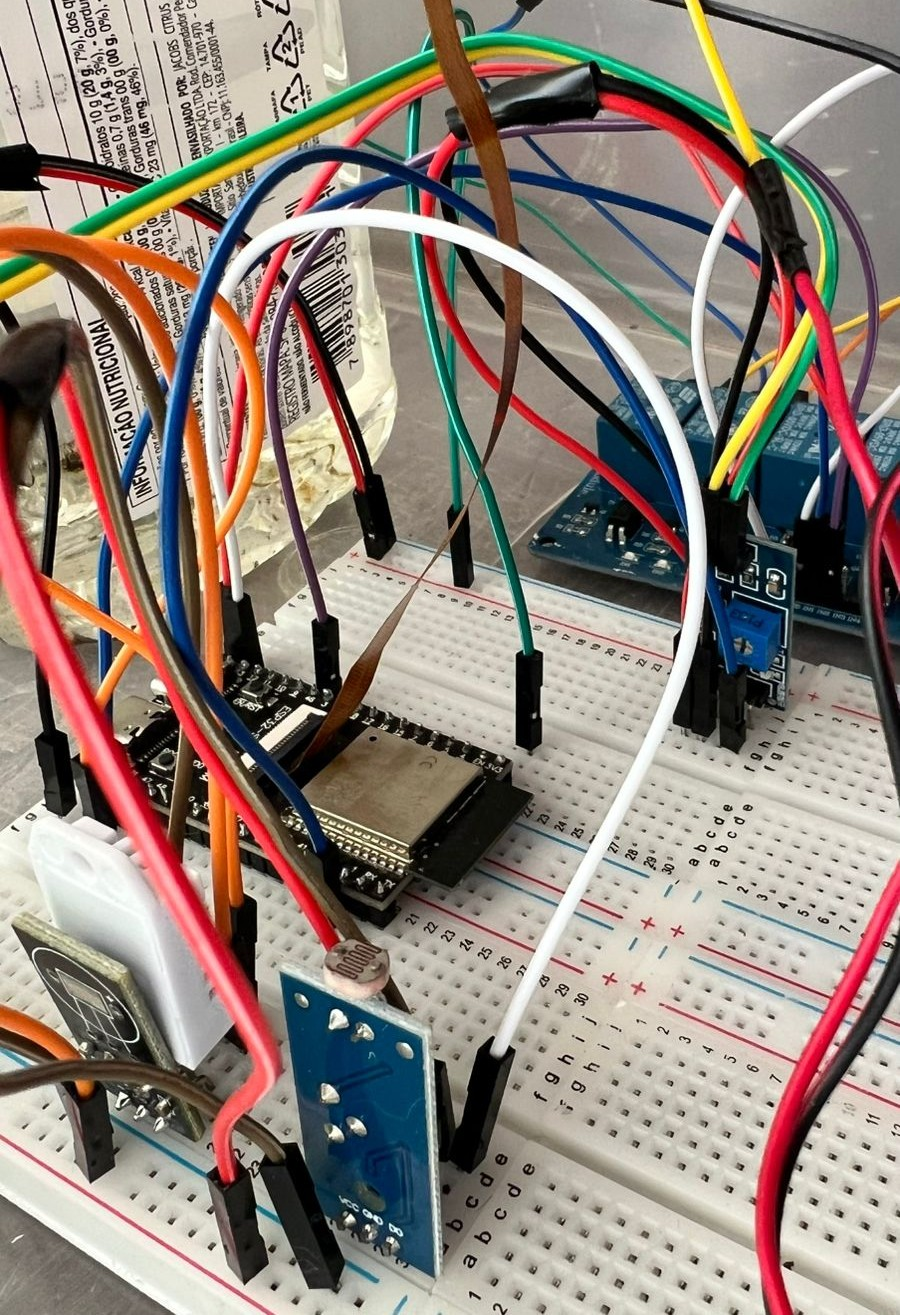
\includegraphics[width=.95\linewidth]{c4.jpeg}\\[-1pt]
  {\small (a) Protótipo físico com \gls{ESP32}-S3, sensores e módulo relé}
\end{minipage}\hfill
\begin{minipage}{.48\textwidth}
  \centering
  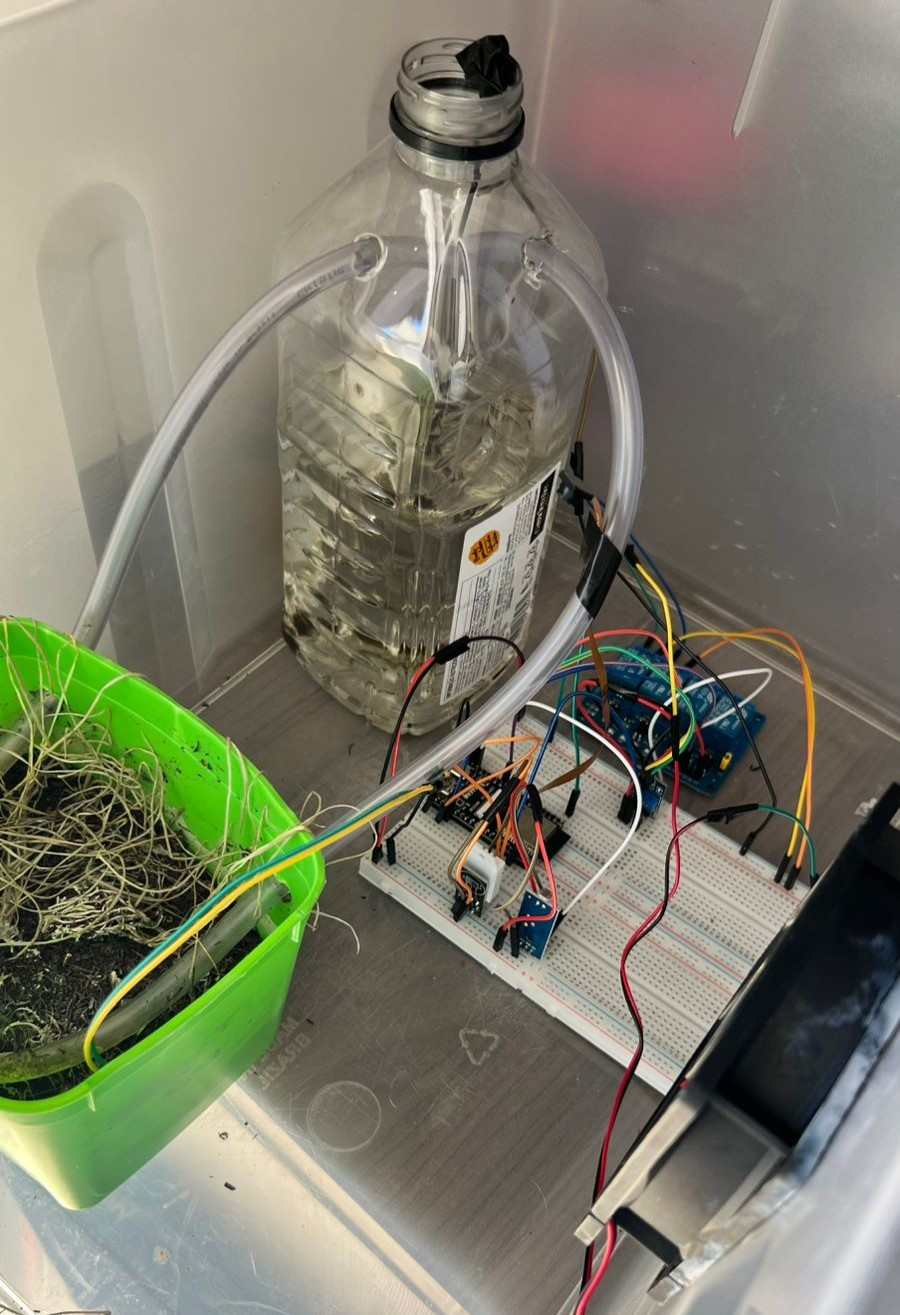
\includegraphics[width=.95\linewidth]{c3.jpeg}\\[-1pt]
  {\small (b) Integração com reservatório e bomba 5V}
\end{minipage}
\caption{Protótipo utilizado nos ensaios.}
\label{fig:proto_duplo}
\end{figure}

\FloatBarrier

\subsection{Validação do controle automatizado}

O firmware executou leituras periódicas e acionou os atuadores conforme a
lógica definida. A bomba foi ativada quando a umidade do solo cruzou o limiar
configurado e desativada após intervalo mínimo, reduzindo reativações por meio
de histerese e temporização. A ventoinha operou em ciclos predefinidos.
Esses achados confirmam o funcionamento autônomo e estável do subsistema
físico durante os ensaios.

\subsection{Interface embarcada e operação do nó}

A Figura~\ref{fig:webui} mostra a interface web embarcada no \gls{ESP32}-S3,
que integra inspeção de sensores e atuadores, histórico de predições e
configuração do servidor, reduzindo a dependência de monitoramento via console
serial e aproximando o fluxo de operação do uso real do dispositivo.

\begin{figure}[ht]
\centering
\begin{minipage}{0.48\linewidth}
    \centering
    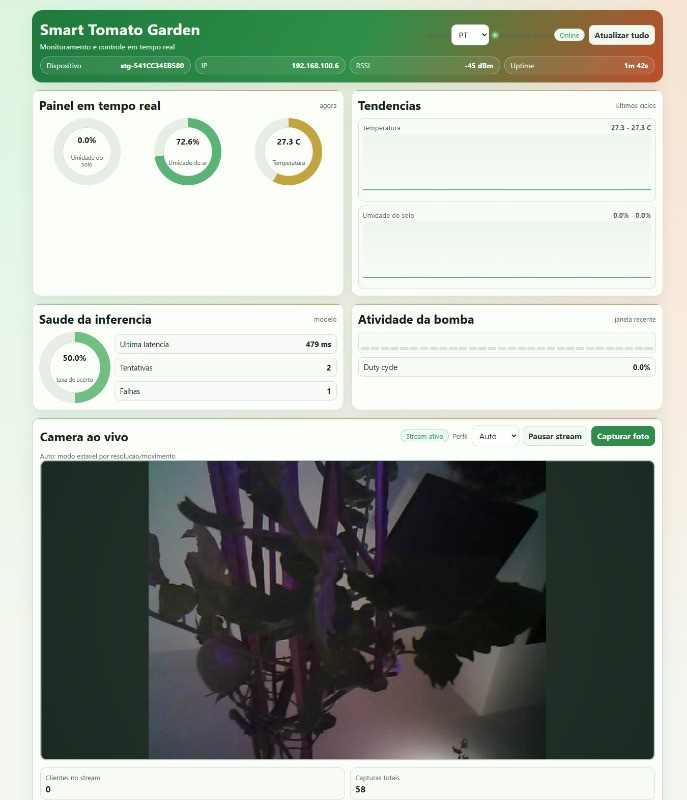
\includegraphics[width=\linewidth]{figuras/interface_web_esp32_1.jpeg}
\end{minipage}\hfill
\begin{minipage}{0.48\linewidth}
    \centering
    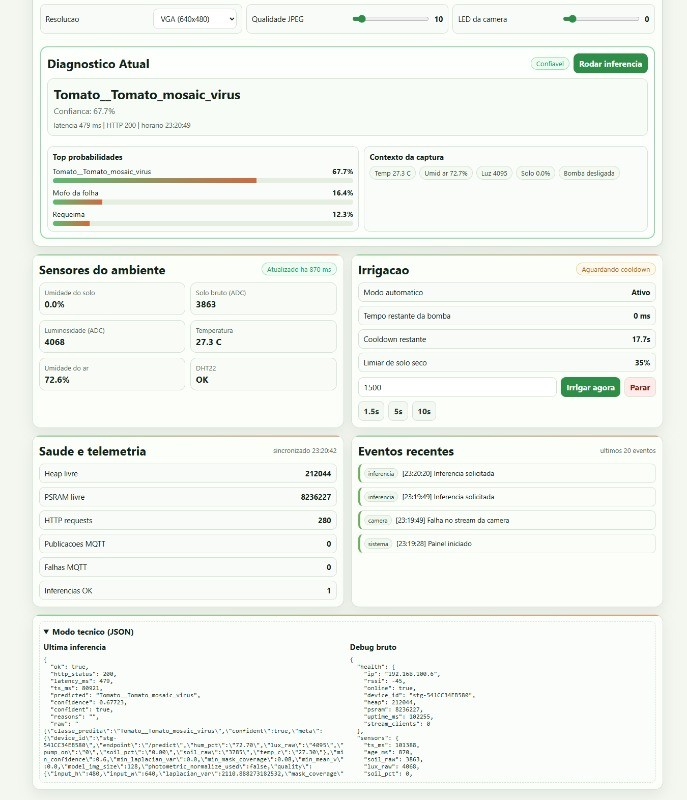
\includegraphics[width=\linewidth]{figuras/interface_web_esp32_2.jpeg}
\end{minipage}
\caption{Interface web embarcada no \gls{ESP32}-S3: à esquerda, monitoramento
dos sensores e estado dos atuadores; à direita, histórico de predições e
configuração do servidor de inferência.}
\label{fig:webui}
\end{figure}

\subsection{Migração do servidor: Python/Flask para Rust/Axum}
\label{sec:migracao}

A migração do backend para Rust foi avaliada em benchmark controlado com
$N = 100$ requisições por servidor (imagens $128 \times 128$\,px, rede local,
10 requisições de aquecimento descartadas), reportando média $\pm$ desvio
padrão, mediana e percentis.

\begin{figure}[ht]
\centering
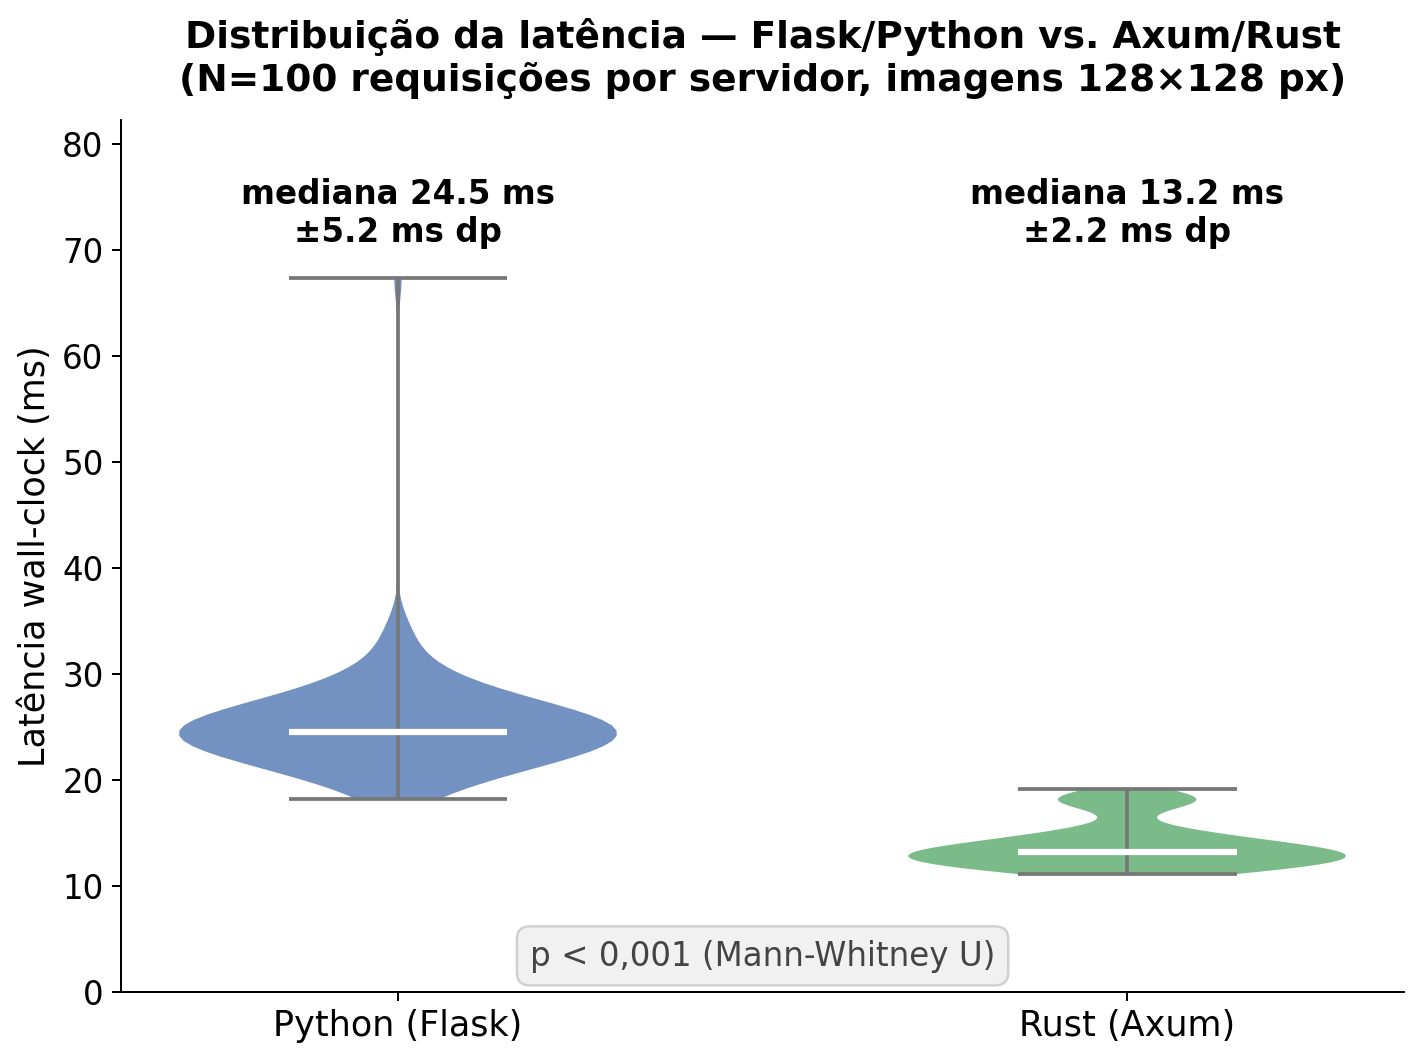
\includegraphics[width=.82\linewidth]{figuras/latency_benchmark_violin.png}
\caption{Distribuição da latência \textit{wall-clock} por servidor
($N=100$ requisições, imagens $128\times128$\,px). A mediana do Rust
(13,2\,ms) é 46\% menor que a do Python (24,5\,ms), com variância
2,4$\times$ menor. Diferença estatisticamente significativa
($p < 0{,}001$, Mann-Whitney~U).}
\label{fig:latency_violin}
\end{figure}
\FloatBarrier

A Figura~\ref{fig:latency_violin} mostra que o servidor Python apresentou
latência \textit{wall-clock} de $25{,}1 \pm 5{,}2$\,ms (mediana 24,5\,ms;
p95 30,5\,ms), enquanto o Rust apresentou $13{,}9 \pm 2{,}2$\,ms (mediana
13,2\,ms; p95 18,3\,ms). A diferença foi estatisticamente significativa
($p < 0{,}001$, Mann-Whitney~U), e o desvio padrão do Rust é 2,4$\times$
menor, indicando latência mais previsível.

A menor variância tem implicação direta no firmware embarcado: um
\textit{timeout} conservador de 50\,ms cobre $>99\%$ das requisições Rust,
enquanto para o Python seria necessário aproximadamente 45\,ms apenas para o
p95. Em cenários com múltiplos nós capturando imagens simultaneamente, a
previsibilidade reduz reenvios por timeout e simplifica a lógica de
\textit{retry} no firmware, contribuindo para a robustez operacional do
sistema em rede local.

\begin{figure}[ht]
\centering
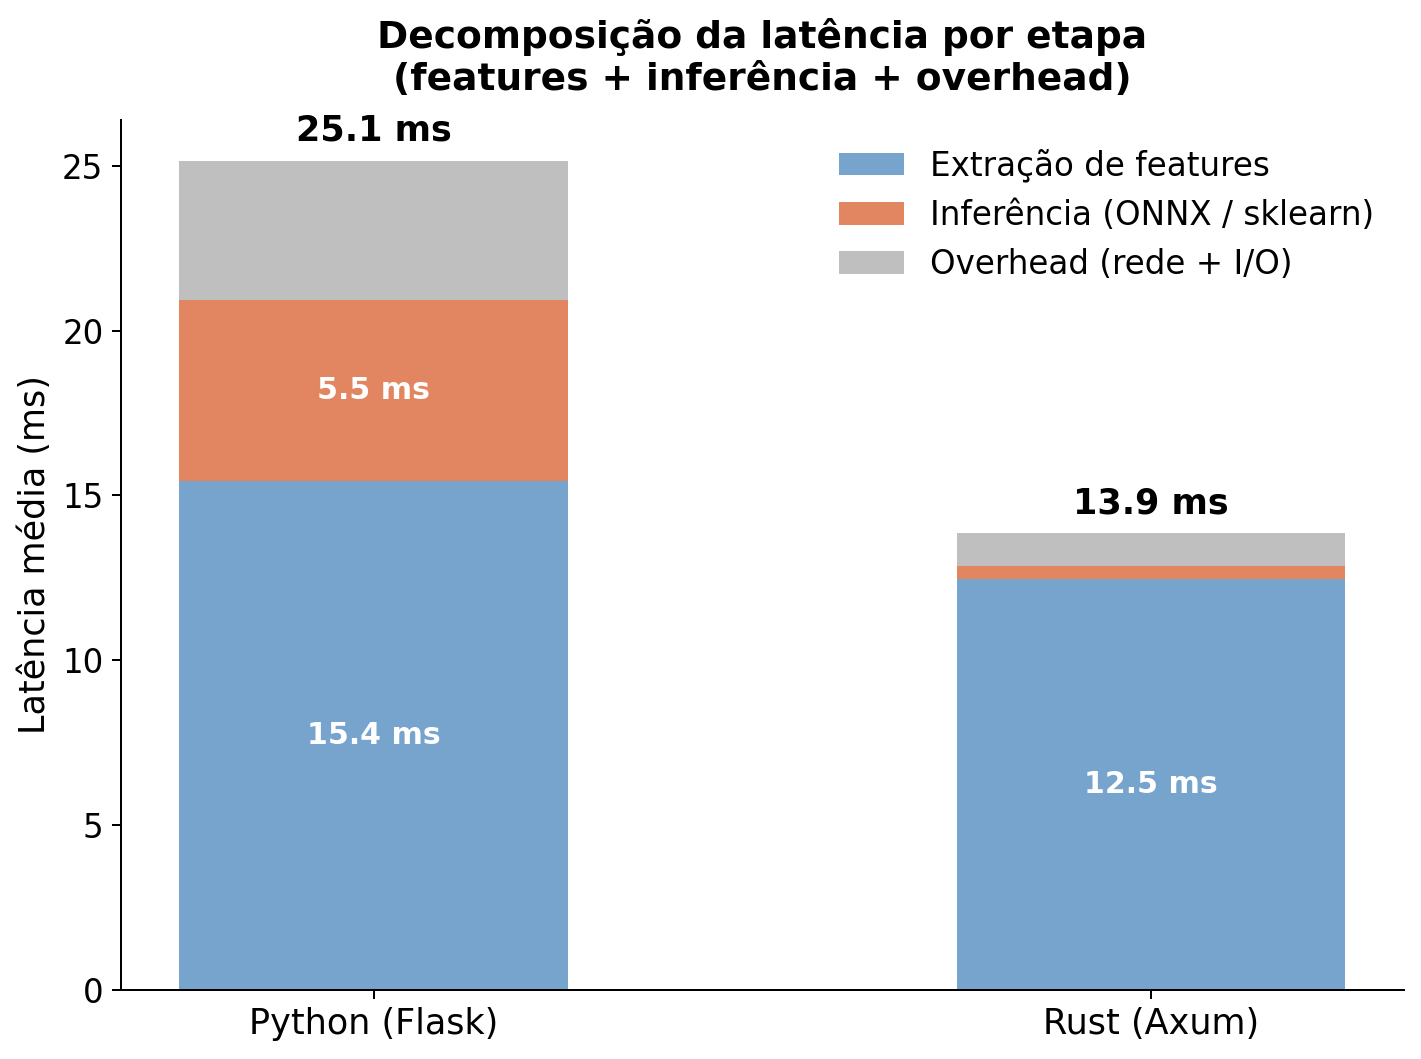
\includegraphics[width=.72\linewidth]{figuras/latency_benchmark_breakdown.png}
\caption{Decomposição da latência média por etapa. A extração de
\textit{features} é similar nas duas implementações (Python: 15,4\,ms;
Rust: 12,5\,ms). O ganho do Rust concentra-se na inferência: ONNX Runtime
(0,4\,ms) é \textbf{14$\times$ mais rápido} que sklearn (5,5\,ms).}
\label{fig:latency_breakdown}
\end{figure}
\FloatBarrier

A Figura~\ref{fig:latency_breakdown} decompõe a latência por etapa: a
extração de atributos é similar nas duas implementações (Python: 15,4\,ms;
Rust: 12,5\,ms), pois ambas executam código nativo nessa etapa --- o Python
delega o cálculo pesado a extensões C (\textit{mahotas}, \textit{scikit-image},
\textit{opencv-python}), evitando o overhead do interpretador, enquanto o
Rust acessa os mesmos algoritmos via \textit{bindings} C++ (\textit{opencv
crate}). O gargalo nessa etapa é algorítmico, não de runtime. O ganho do
Rust concentra-se inteiramente na inferência: ONNX Runtime (0,4\,ms) é
\textbf{14$\times$ mais rápido} que sklearn (5,5\,ms).

O ganho concentrado na inferência tem explicação arquitetural: o sklearn,
mesmo utilizando XGBoost implementado em C internamente, atravessa a
fronteira Python\,$\rightarrow$\,C a cada chamada de \texttt{predict()},
com alocação de arrays numpy e aquisição do GIL. O ONNX Runtime executa um
grafo de computação pré-compilado diretamente em C++, sem overhead de
runtime interpretado, eliminando essas transições.

A decomposição evidencia que a extração de atributos tornou-se o gargalo
dominante no servidor Rust: os 12,5\,ms de extração representam 90\% da
latência mediana total (13,9\,ms). Esse resultado indica que otimizações
adicionais devem focar nessa etapa --- por exemplo, paralelização de grupos
de descritores independentes (Haralick, Zernike e LBP podem ser computados
concorrentemente) ou substituição parcial dos descritores manuais por
representações aprendidas de uma \gls{CNN} leve, o que reduziria também a
dependência de bibliotecas C externas em tempo de implantação.

\begin{figure}[ht]
\centering
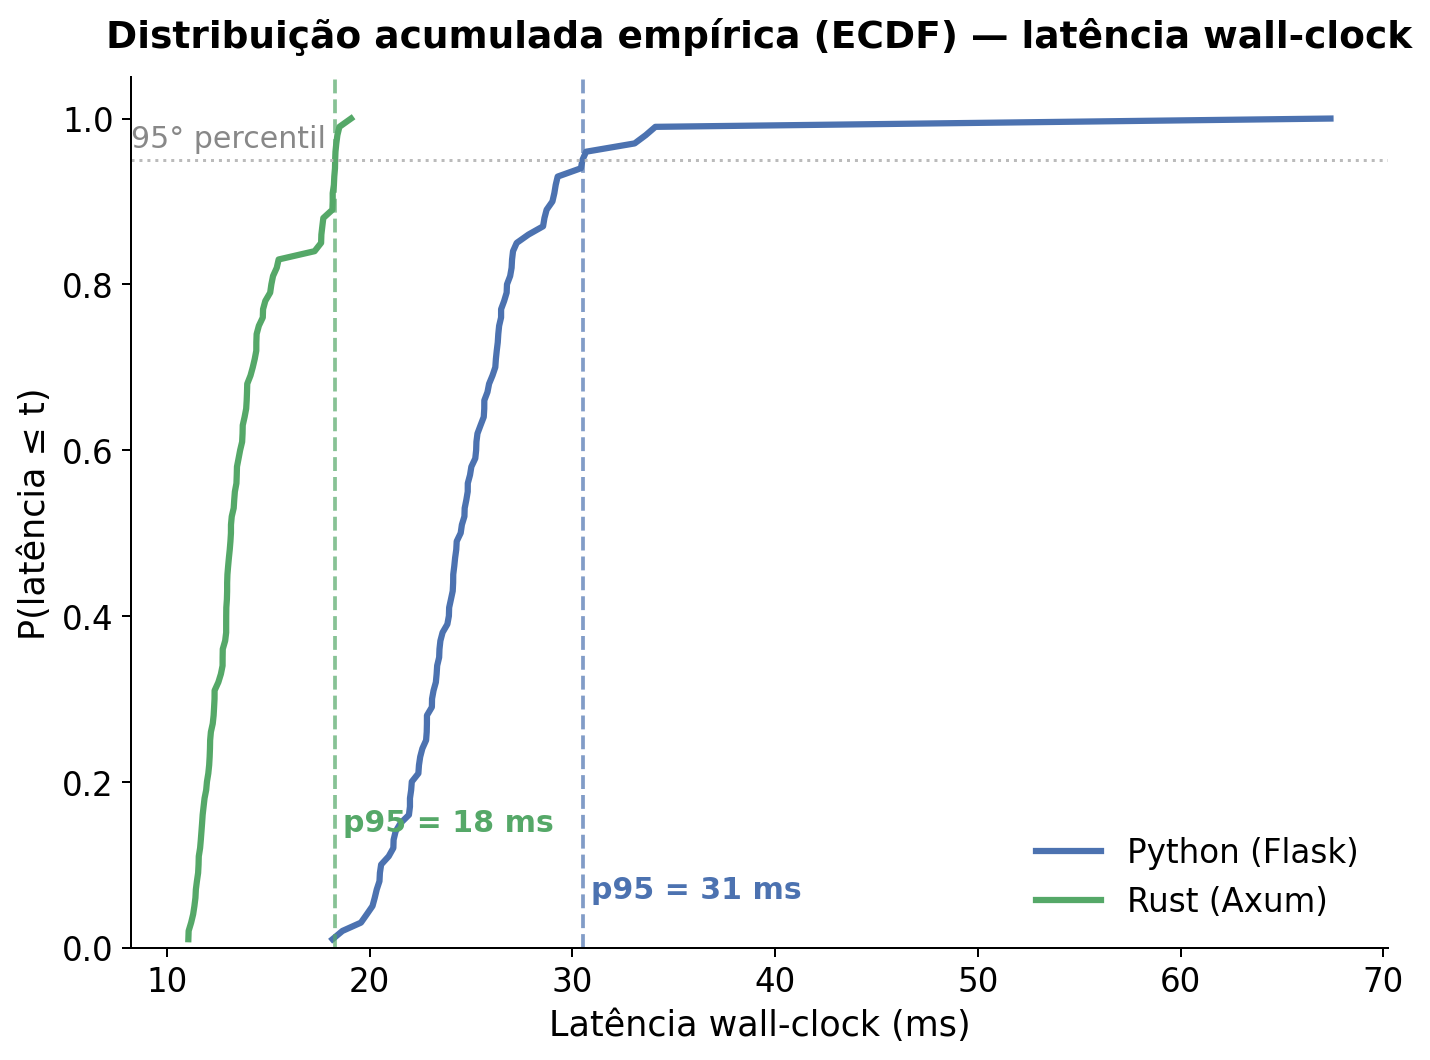
\includegraphics[width=.82\linewidth]{figuras/latency_benchmark_ecdf.png}
\caption{Função de distribuição acumulada empírica (ECDF) da latência
\textit{wall-clock}. O $95^\circ$ percentil do Rust (18\,ms) é inferior
à mediana do Python (24,5\,ms), indicando que mesmo os piores casos do
Rust são melhores que o comportamento típico do Python.}
\label{fig:latency_ecdf}
\end{figure}
\FloatBarrier

A Figura~\ref{fig:latency_ecdf} reforça esse resultado: o $95^\circ$
percentil do Rust (18\,ms) é inferior à própria mediana do Python
(24,5\,ms), mostrando que mesmo os piores casos do Rust superam o
comportamento típico do Python.

Além do ganho de latência, o consumo de memória em repouso cai para
$\sim$38\,MB (vs.\ $\sim$210\,MB do stack Python/Flask, redução de 82\%).
Essa diferença tem impacto direto no espaço de implantação possível: somado
ao consumo do sistema operacional ($\sim$80--100\,MB em Raspberry Pi OS
Lite), o stack Python deixa apenas $\sim$200\,MB livres no Raspberry Pi
Zero~2W (512\,MB), operando no limite sob carga de processamento de imagem.
O backend Rust, com 38\,MB de baseline, preserva mais de 370\,MB
disponíveis, viabilizando execução estável no mesmo hardware sem
comprometer outros processos do gateway. O binário autocontido
($\sim$27\,MB) dispensa gerenciamento de runtime e suporta distribuição via
OTA sem dependências de sistema --- o que, combinado ao
\textit{cross-compilation} para ARM, viabiliza atualizações em frotas de
nós distribuídos sem intervenção manual.

A transição foi validada via \textit{shadow mode}: execução paralela das
duas implementações com comparação de respostas antes do corte definitivo.
Esse protocolo de validação de migração é raramente documentado em trabalhos
acadêmicos de agricultura de precisão, sendo uma contribuição metodológica
para reprodutibilidade que outros grupos podem adotar ao migrar sistemas de
prototipagem para produção.

\FloatBarrier

\subsection{Inferência com imagens reais e sensibilidade à iluminação}

A câmera \gls{OV2640} operou com captura local via WiFi e envio de imagens
ao servidor em Rust via \gls{HTTP}. Em testes com imagens capturadas pelo
protótipo, o serviço retornou a classe predita, pontuação, lista
\textit{top-k}, tempos por etapa e indicadores de qualidade. A latência
mediana fim a fim --- incluindo transmissão WiFi --- ficou em torno de
26\,ms, compatível com aplicações próximas ao tempo real em rede local.

\begin{figure}[ht]
\centering
\begin{minipage}{.48\textwidth}
  \centering
  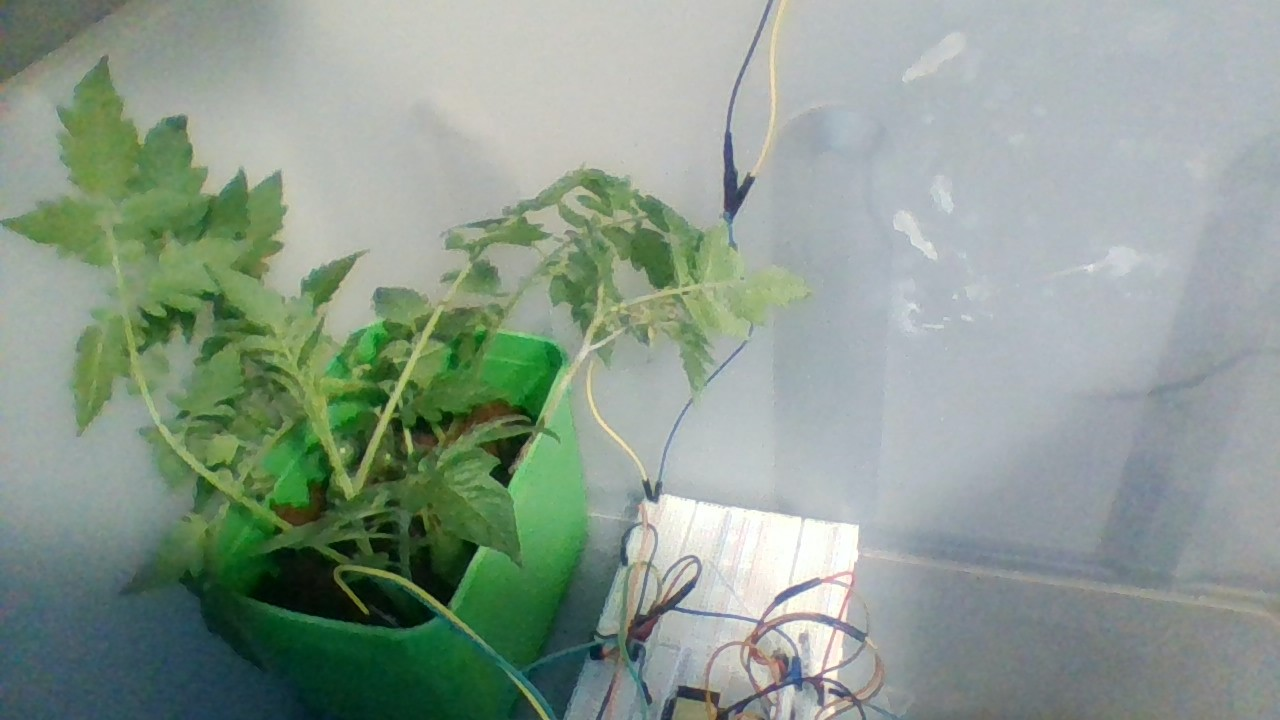
\includegraphics[width=.95\linewidth]{resultado1.jpg}\\[-1pt]
  {\small (a) Imagem real}
\end{minipage}\hfill
\begin{minipage}{.48\textwidth}
  \centering
  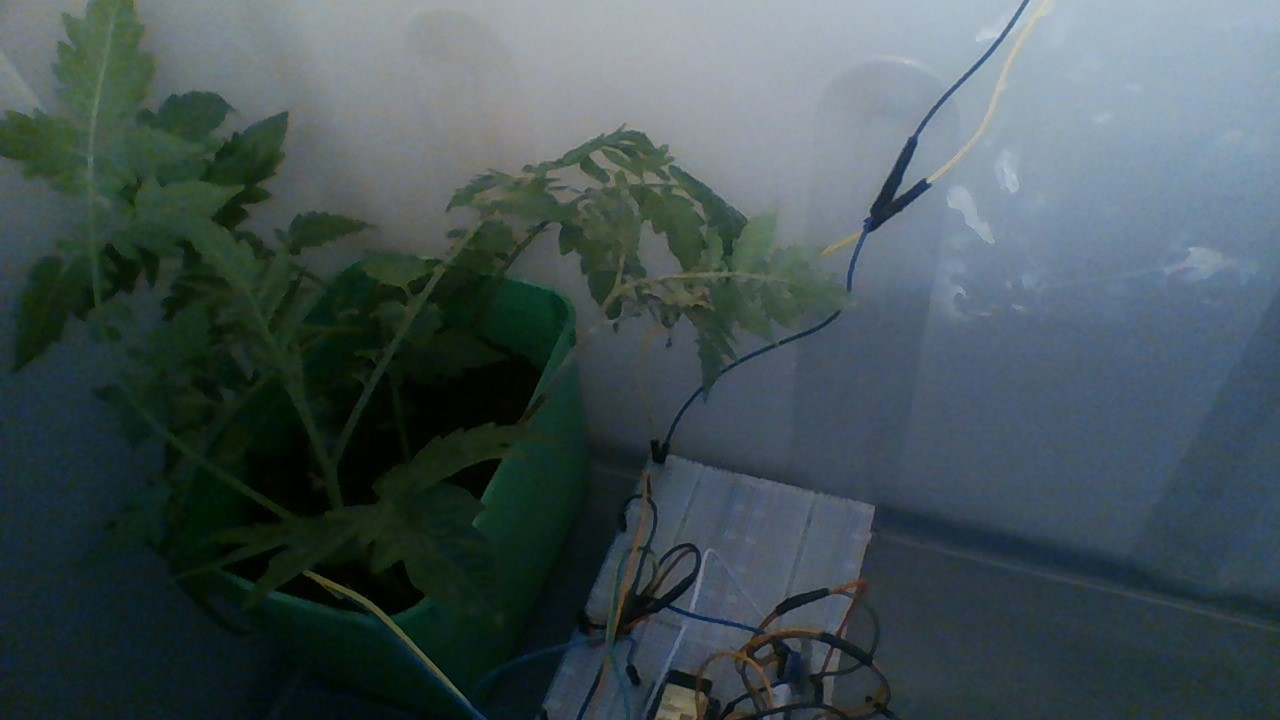
\includegraphics[width=.95\linewidth]{resultado3.jpg}\\[-1pt]
  {\small (b) Imagem real mais escura}
\end{minipage}
\caption{Exemplos \emph{in situ} capturados pelo sistema.}
\label{fig:res_real_duplo}
\end{figure}

A resposta do servidor inclui a classe predita, pontuação, tempos por etapa,
indicadores de qualidade e a sinalização de confiança. Em imagens mais escuras ou com menor nitidez,
observou-se maior ambiguidade no \textit{top-k}, consistente com a
dependência dos descritores de cor e textura em condições fotométricas
desfavoráveis. Os \textit{quality gates} --- cobertura de máscara e variância
do Laplaciano --- sinalizam nesses casos a necessidade de reaquisição.

\medskip\noindent\textbf{Sensibilidade à iluminação e mitigação.}
Em avaliação controlada com escurecimento simulado ($\gamma = 1{,}4$), a
macro F1 caiu de 96,19\% para 90,11\%; com redução de brilho de 20 unidades,
para 91,57\%, confirmando a dependência dos descritores de cor em condições
fotométricas adversas. Como medidas práticas destacam-se: iluminação auxiliar
e ajuste de exposição/\textit{gain}; \textit{data augmentation} orientada a
variações de brilho e contraste; e reaquisição condicionada por
\textit{quality gates} quando a imagem estiver fora de faixa.

\FloatBarrier

\subsection{Comparação entre classificadores clássicos e baseline profunda}
\label{sec:classificadores}

Para contextualizar a escolha do XGBoost, os três classificadores clássicos
foram treinados sobre o \emph{mesmo} vetor de 188 atributos, com o
\emph{mesmo} protocolo de particionamento (\textit{StratifiedGroupKFold}) e
avaliados no mesmo conjunto de teste independente de 4.803 amostras.
A Figura~\ref{fig:classifier_comparison} sintetiza os resultados.

\begin{figure}[ht]
\centering
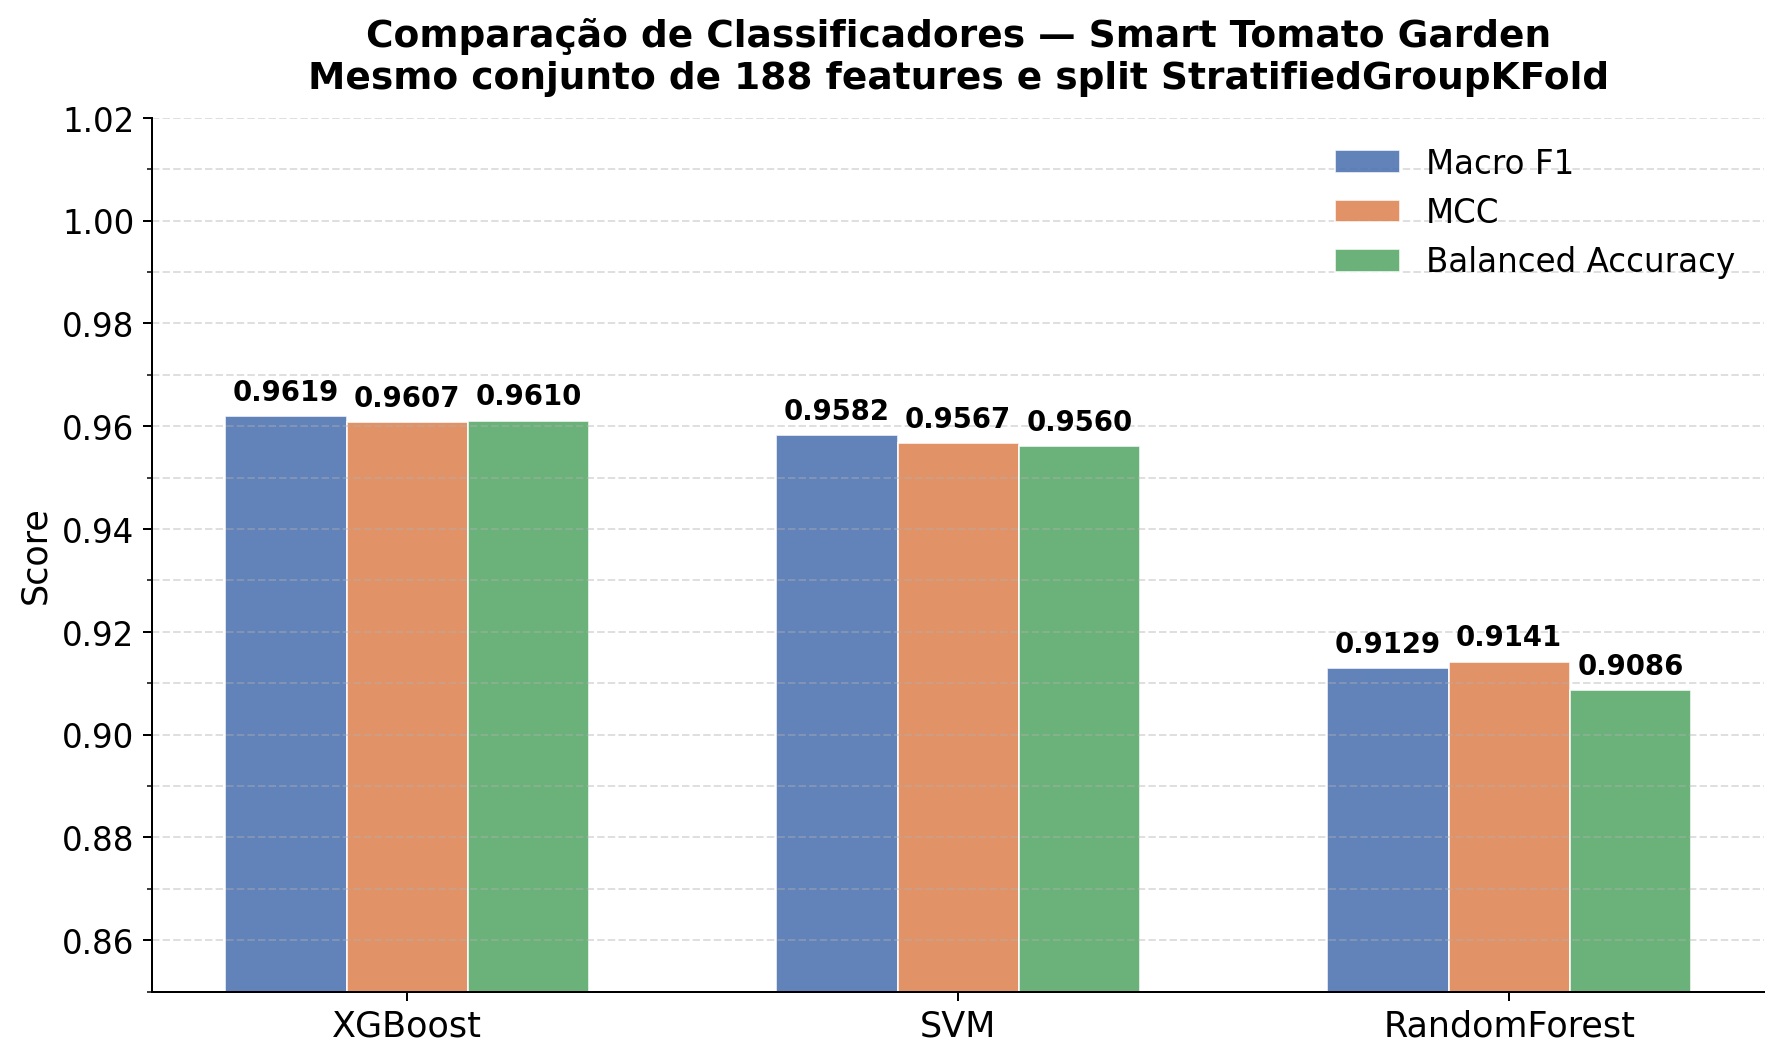
\includegraphics[width=.92\linewidth]{figuras/classifier_comparison.png}
\caption{Comparação entre XGBoost, SVM e Random Forest em Macro F1, MCC e
\textit{Balanced Accuracy}. Todos os classificadores foram avaliados sobre
os mesmos 188 atributos e o mesmo conjunto de teste.}
\label{fig:classifier_comparison}
\end{figure}

O XGBoost superou o SVM em macro F1 ($+0{,}37$\,p.p.) e o Random Forest em
$+4{,}9$\,p.p., confirmando que a escolha é empiricamente justificada dentro
do espaço de classificadores clássicos para este conjunto de atributos. O SVM
(RBF, $C=10$, \textit{gamma=auto}) apresenta desempenho próximo ao XGBoost e
constitui alternativa viável quando interpretabilidade das árvores não é
requisito. O Random Forest, apesar da macro F1 de 91,29\%, oferece vantagem em
velocidade de treinamento ($\sim$6$\times$ mais rápido), tornando-o adequado
para iterações exploratórias.

Os resultados mostram dois perfis complementares. O pipeline clássico com
atributos interpretáveis (XGBoost: 96,19\%) permite análise direta dos sinais
de cor, textura e forma associados às classes, com custo computacional
compatível com atualização frequente do modelo. A MobileNetV3-Small (99,02\%)
obtém macro F1 superior ao aprender representações de ponta a ponta, porém
com menor transparência interna. Em um sistema embarcado com forte componente
de engenharia aplicada, esse equilíbrio entre interpretabilidade, desempenho e
viabilidade de implantação é particularmente relevante.

A análise por classe (Tabela~\ref{tb:perclass}) reforça essa leitura. As
maiores dificuldades do XGBoost concentram-se em \textit{Early Blight}
(90,43\%) e \textit{Target Spot} (94,95\%), consistente com a maior
sutileza visual de lesões iniciais ou necrosantes. Classes como
\textit{Healthy} (98,44\%) e \textit{Yellow Leaf Curl} (98,13\%) mantiveram
desempenho elevado.

\begin{table}[ht]
\caption{F1-score por classe --- XGBoost + 188 \textit{features} (conjunto de
teste, 4.803 amostras)}
\label{tb:perclass}
\centering
\setlength{\tabcolsep}{5pt}
\renewcommand{\arraystretch}{1.1}
\begin{tabularx}{\textwidth}{Y c c c}
\toprule
\textbf{Classe} & \textbf{Precisão} & \textbf{Recall} & \textbf{F1} \\
\midrule
Bacterial Spot      & 97,51\% & 98,12\% & 97,81\% \\
Early Blight        & 94,55\% & 86,67\% & 90,43\% \\
Late Blight         & 95,28\% & 95,28\% & 95,28\% \\
Leaf Mold           & 96,82\% & 95,80\% & 96,31\% \\
Septoria Leaf Spot  & 95,91\% & 97,18\% & 96,54\% \\
Spider Mites        & 95,86\% & 96,62\% & 96,24\% \\
Target Spot         & 93,95\% & 95,96\% & 94,95\% \\
Yellow Leaf Curl    & 98,43\% & 97,82\% & 98,13\% \\
Mosaic Virus        & 97,35\% & 98,21\% & 97,78\% \\
Healthy             & 97,53\% & 99,37\% & 98,44\% \\
\bottomrule
\end{tabularx}
\end{table}

\section{Conclusão}

Este trabalho apresentou o desenvolvimento e a validação de uma horta indoor
que integra automação agrícola, \gls{IoT} e \gls{IA} para monitoramento
ambiental e diagnóstico de doenças foliares em tomateiro. A solução combinou
sensores e atuadores controlados por \gls{ESP32}-S3, firmware com interface
web e configuração persistente, e um serviço de inferência em Rust/Axum com
ONNX Runtime.

Entre os classificadores clássicos avaliados sobre o mesmo vetor de 188
atributos, o XGBoost obteve o maior macro F1 de 96,19\% (MCC 0,9607),
superando SVM ($+0{,}37$\,p.p.) e Random Forest ($+4{,}9$\,p.p.). A
MobileNetV3-Small atingiu 99,02\% como teto de desempenho com aprendizado de
ponta a ponta.

No plano operacional, o benchmark controlado ($N = 100$) demonstrou que o
backend Rust reduz a latência mediana para 13,2\,ms (vs.\ 24,5\,ms do
Python), com ganho de $14\times$ na etapa de inferência ONNX Runtime vs.\
sklearn e redução de 82\% no consumo de memória em repouso (38\,MB vs.\
210\,MB). Esse footprint viabiliza a execução do serviço diretamente em
hardware de borda como Raspberry Pi Zero~2W, eliminando a dependência de
servidor externo e aproximando o sistema de implantação totalmente autônoma em
campo.

Como limitação principal, a validação dos modelos depende integralmente do
PlantVillage, conjunto com características controladas. Imagens coletadas
diretamente pelo protótipo em condições naturais de campo são ainda
insuficientes para avaliação estatística robusta da validade externa dos
modelos.

Como trabalhos futuros, destacam-se: (i) expansão do conjunto de imagens
coletadas \emph{in situ} para validação em condições reais diversas; (ii)
refinamento de estratégias de rotulagem por estágio ou fenótipo; (iii)
execução totalmente \emph{on-device} no gateway sem servidor externo,
viabilizada pelo footprint de 38\,MB do backend Rust; (iv) \textit{cross-compilation}
do binário Rust para ARM (Raspberry Pi) e distribuição por OTA em frotas
distribuídas; e (v) avaliação de modelos quantizados compatíveis com
inferência diretamente no ESP32-S3.

\bibliographystyle{sbc}
\bibliography{sbc-template}

\end{document}
